\begin{refsection}
%-------------------------------------------------------------------------
%-------------------------------------------------------------------------
\chapter{Measuring optical imperfections in refractive lenses}\label{sec:measuring}
%-------------------------------------------------------------------------
%-------------------------------------------------------------------------

Surface metrology methods commonly applied to X-ray mirrors [\cite{Alcock2016, Vivo2019}] are not broadly employed for the metrology of X-ray lenses mainly due to their small apertures and steep parabolic surfaces (cf. Fig.~\ref{fig:ideal_CRL}) [\cite{Lyatun2015}]. Non-destructive methods using X-rays are often more appropriate for X-ray lens metrology. This section presents some of the commonly used at-wavelength metrology methods, with emphasis on X-ray speckle vectorial tracking (XSVT), the experimental technique used throughout this work. The metrology of single- and stacked 2D-Beryllium lens with $R=50~\mu$m is presented and the results are compared. %A framework for calculating corrective optics for such stacked lenses is shown, along with the first correction prototypes and tests.

The experimental data shown in this chapter were acquired on several beamtimes\footnote{Acknowledgements to Sébastien Bérujon and Ruxandra Cojocaru (BM05-ESRF); Xianbo Shi, Zhi Qiao, Michael Wojcik and Lahsen Assoufid (1-BM-APS); and to Carsten Detlefs (ID06-ESRF) for the help during the experimental sessions.} at the BM05 beamline - ESRF [\cite{Ziegler2004}] (from 2017 to 2018 - before the ESRF long shutdown for the EBS upgrade), at the 1-BM beamline - APS [\cite{Macrander2016}] (in 2019 during the ESRF long shutdown) and the ID06 beamline - ESRF [\cite{Kutsal_2019}] (in 2020 in the commissioning period of the ESRF-EBS upgrade).


%-------------------------------------------------------------------------
%-------------------------------------------------------------------------
\section{At wavelength-metrology}\label{sec:at_wavelength}
%-------------------------------------------------------------------------
%-------------------------------------------------------------------------

Surface metrology of X-ray optical elements is often done using visible spectral range [\cite{Alcock2016, Vivo2019}] even if, ultimately, they will be employed in a different spectral range. At-wavelength metrology is an umbrella term for measurements of optical elements at wavelengths closer to the ones they will be ultimately used - in the case of X-ray lenses, in the range of few to several kilo-electron-volts. What follows is a non-exhaustive description of commonly used techniques for quality control applied to X-ray lenses and their compliance to a parabolic shape. Other relevant at-wavelength characterisations of X-ray lenses such as X-ray small-angle scattering [\cite{Roth2014, Chubar2020}] or the impact of material micro-structures or shape errors on imaging [\cite{Chubar2020,Lyatun2020}] are not covered here. 

The simplest at-wavelength techniques consist of the direct imaging of a lens with X-rays by propagation-based phase-contrast imaging [\cite{Endrizzi2018}], since absorption contrast imaging only generates a reduced contrast for a single lens and a low signal to noise ratio. With such simple techniques, 2D shapes and distances can be measured (e.g. radiographs for controlling the distance and alignment between the parabolic surfaces of X-ray lenses). Still based on propagation based-imaging techniques, X-ray laminography [\cite{Helfen2011,Roth2014}] and X-ray tomography [\cite{Landis2010,Narikovich2017}] of X-ray lenses provide a 3D reconstruction of the lens volume with high spatial resolution information. These techniques provide data on the shape of the refracting surfaces and the internal features (inhomogeneities) and can be used for modelling optical imperfections in refractive lenses. 


Another large family of experimental techniques used for lens metrology and aiming at quantitative optical characterisation can be grouped under the wave-front sensing branch\footnote{With the advent of more coherent sources of X-rays as encapsulated by the emergence of $4^{\text{th}}$-generation synchrotrons and free-electron lasers, the topic of wavefront sensing has seen increased attention [\cite{Seaberg2019}].}. Wavefront-sensing is often employed as a beam-diagnostics tool for highly coherent sources [\cite{Seaberg2019}]. Two conceptual approaches are often used: \textit{i}-) absolute wavefront metrology at a specific point of the beam path measures the global state of the wavefront or \textit{ii}-) differential measurements are done with and without the optical element under investigation, the differences in the wavefront being attributed to the optical contribution of the element under test. Current wavefront-sensing techniques used so far in the community for evaluating the phase errors of CRLs (or individual X-ray lenses) are: the Ronchi test, an interferometric technique that provides qualitative\footnote{It has been demonstrated that the Ronchi test can also retrieve quantitative information [\cite{Lee2010}], but it has not yet been applied to X-ray lenses metrology.} information on third-order optical aberrations [\cite{Nilsson2012, Uhlen2014}]; the use of X-ray Shack–Hartmann sensors [\cite{Mayo2004, Mercere2005, Mikhaylov2020}]; the ptychographic reconstruction of the wavefront emerging from a strong focusing optics [\cite{Schropp2013,Sala2017,Seiboth2017}]; grating interferometry and its variations [\cite{David2012,Koch2016,Grizolli2017}]; and the near-field-speckle-imaging-based (SBI) methods [\cite{Berujon2013,Zdora2018,Berujon2020a}]. The latter is the main experimental technique used in this project and the remaining of this chapter will focus more deeply on its theoretical and experimental aspects.


%-------------------------------------------------------------------------
%-------------------------------------------------------------------------
\subsection{X-ray (near field) speckle vector tracking (XSVT)}\label{sec:XSVT}%\addcontentsline{toc}{subsection}{-- X-ray (near field) speckle vector tracking (XSVT)}
%-------------------------------------------------------------------------
%-------------------------------------------------------------------------

The X-ray near-field-speckle-imaging is currently the chosen technique for systematic at-wavelength metrology of X-ray lenses at the ESRF\footnote{Other synchrotron facilities also offer X-ray lens metrology with the X-ray near field speckle imaging technique: 1-BM at the APS in the U.S.A. [\cite{Qiao2020}] and the B16 beamline at the Diamond Light Source in the U.K. [\cite{Sawhney2013}].} and is available at the BM05 beamline [\cite{Berujon2020a}] and most recently, at the ID06 beamline. The principal reasons for this choice are: \textit{i}-) the low requirements on transverse- and longitudinal coherence [\cite{Zanette2014,Zdora2015,Wang2016}]; \textit{ii}-) no requirement of specially tailored optics (nor accompanying complicated alignment procedures) [\cite{Morgan2012,Wang2016}]; \textit{iii}-) successful benchmark against more established wave-front sensing techniques [\cite{Kashyap2016,Romell2017}]; and \textit{iv}-) its versatility as a metrology tool being able to measure mirrors, single- and stacked lenses [\cite{Berujon2020a}]. Although the basic principles of the several X-ray near-field-speckle-based techniques are the same, the focus is given here to the X-ray (near field) speckle vector tracking (XSVT) as implemented and used for the metrology of single- and stacked X-ray lenses used in this work [\cite{Berujon2020a,Berujon2020}]. An interesting review of different techniques using X-ray near-field speckle imaging is given by [\cite{Zdora2018a}] and [\cite{Berujon2020}].

%-------------------------------------------------------------------------
%-------------------------------------------------------------------------
\subsection{Foundation}\label{sec:foundation}
%-------------------------------------------------------------------------
%-------------------------------------------------------------------------

Near-field speckle is a manifestation in intensity of the summation of several complex electric fields when the amplitudes and phases of such fields have random values. The resulting intensities may be locally high due to constructive interference or low, due to destructive interference [\cite[\textit{\S1}]{Goodman2020}]. For a speckle pattern over a defined region of interest, the speckle contrast (or visibility) can be defined\footnote{Other definitions are commonly found in the literature: $v=\frac{I_\text{max}-I_\text{min}}{I_\text{max}-I_\text{min}}$ and $v=\frac{I_\text{max}-I_\text{min}}{2\overline{I}}$, where $I_\text{max}$ and $I_\text{min}$ are the maximum and minimum intensities found in the region of interest [\cite{Zdora2018a}].} as:
\begin{equation}\label{eq:visibility}
    v=\frac{\sigma_I}{\overline{I}},
\end{equation}
where $\sigma_I$ is the standard deviation and $\overline{I}$ is the mean value of the intensity value of the speckle pattern. In the X-ray regime, it appears when a sufficiently coherent X-ray beam is transmitted through matter with random spatial variation of $\delta$ and $\beta$, where the local optical path length varies significant when compared to the scale of the wavelength.

For a static random modulation of the wavefield (stationary diffuser\footnote{As opposed to time-varying modulation of the speckle-field as in [\cite{Morgan2010,Goikhman2015}].}), it has been demonstrated that the speckle-grains\footnote{Continous regions in space with a slowly-varying intensity that can be visually clustered together.} preserve shape and size for free-space propagation distances limited to:
\begin{equation}\label{eq:speckle_goodness}
z<\Delta_{\textbf{cl}_\perp}\xi k,
\end{equation}
where $\Delta_{\textbf{cl}_\perp}$ is transverse coherence length\footnote{cf. \textit{Spatial coherence} in \S\ref{sec:optical_coherence}~-~\textit{\nameref{sec:optical_coherence}}.} and $\xi$ is the typical transverse length of the modulator, that is, the region where the spatial variation of $\delta$ and $\beta$ is negligible [\cite{Cerbino2008}]. For propagation distances smaller than the imposed limit in Eq.~\ref{eq:speckle_goodness}, speckles can be used as a wavefront marker, since the transverse position of the speckle grains in two parallel planes along the propagation direction can be inferred geometrically. The near-field regime is of particular interest for the X-ray energy range, as very low wavelengths lead to an extended near-field regime. A speckle-pattern and the stationary diffuser used to generate it are shown in Fig.~\ref{fig:SpecklePattern}.

\begin{figure}[t]
        \centering
        {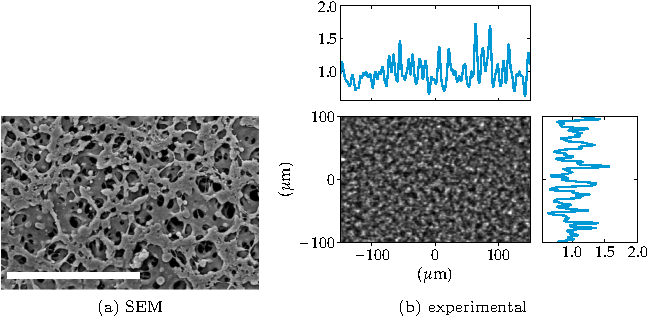
\includegraphics[width=0.6\linewidth]{figures/ch04/SpecklePattern.pdf}}
        \caption[Speckle-pattern and the stationary diffuser]{(a) Speckle-pattern measured at 17~keV at 800~mm downstream the with $\sigma_I=0.19$~a.u., $\overline{I}=0.99$~a.u. and $v\sim0.19$; (b) SEM image of the cellulose acetate membrane filters with mean pore size of 1.2~$\mu$m used as the stationary diffuser. The white bar in (b) represents 50~$\mu$m.} \label{fig:SpecklePattern}
\end{figure}

\begin{figure}[t]
        \centering
        {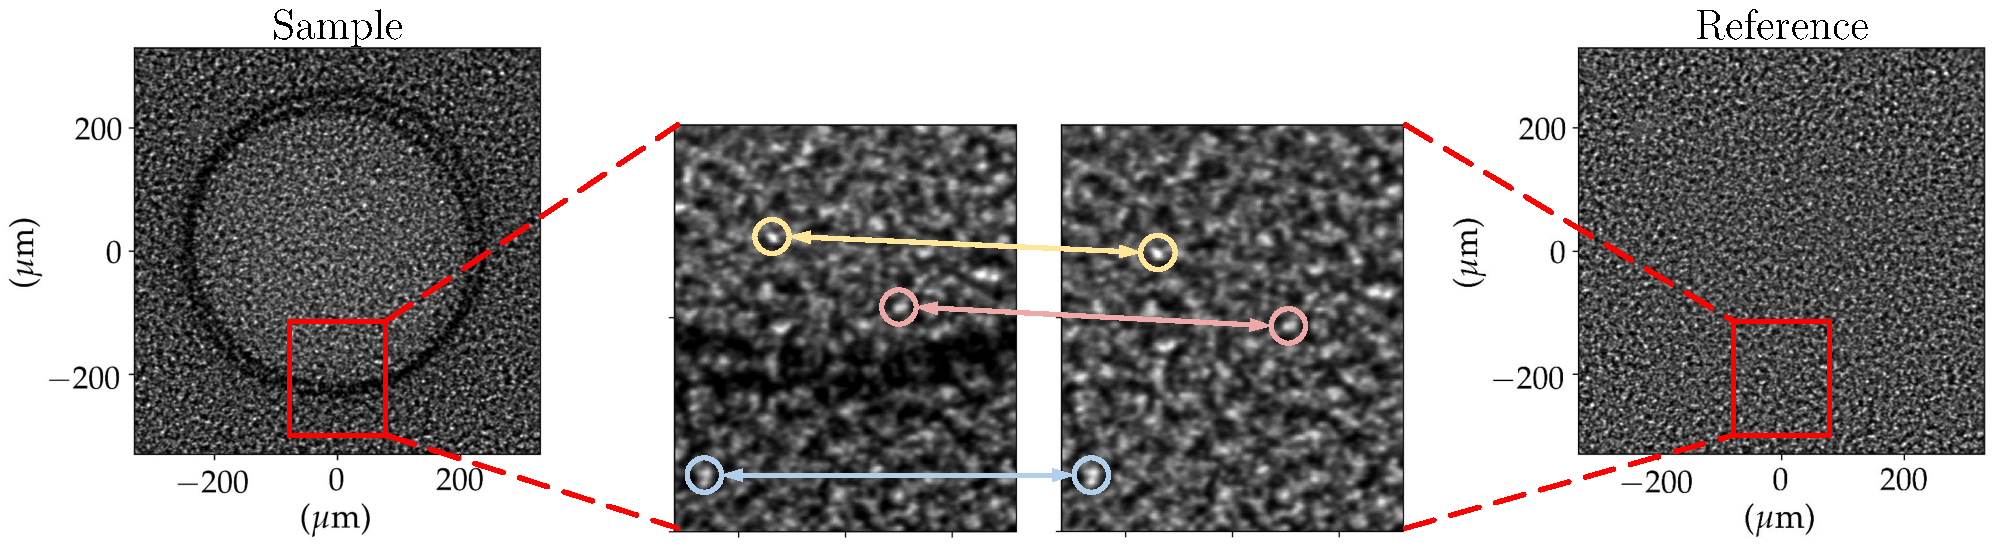
\includegraphics[width=1\linewidth]{figures/ch04/speckle_tracking.pdf}}
        \caption[Tracking of speckle grain]{Tracking of speckle grains. The highlighted grains in yellow and red are inside the sample and have their transverse position changed. The highlighted grain in blue is outside the lens active area and has no apparent shift in the transverse position. The speckle grains in the image of the sample have their intensity reduced due to absorption of the bulk material. The sample is a single 2D-Beryllium lens with nominal radius $R=50~\mu\text{m}$, geometric aperture $A_{\diameter}\sim440$~\textmu m. The data were collected $\sim$800mm downstream the speckle-membrane at 17~keV.} \label{fig:speckle_tracking}
\end{figure}

\begin{figure}[t]
        \centering
        {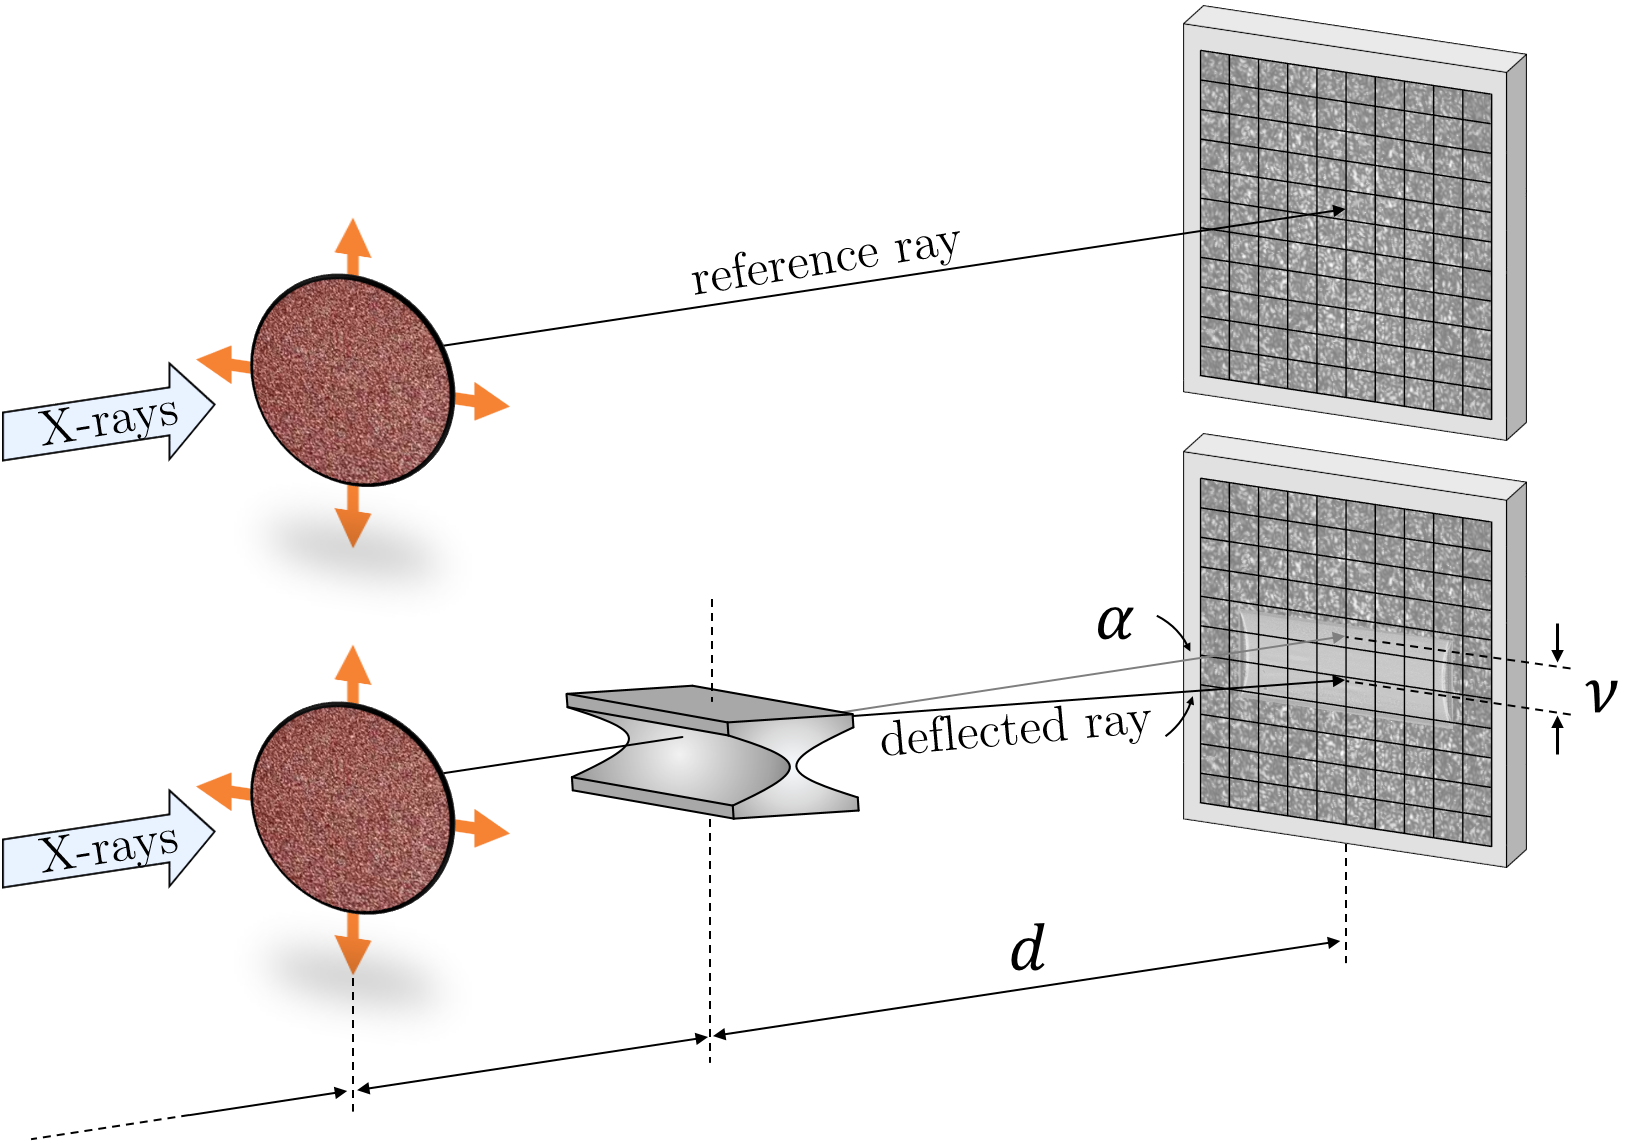
\includegraphics[width=0.6\linewidth]{figures/ch04/speckle_tracking2.png}}
        \caption[Speckle-based imaging geometry]{Generic speckle-based imaging measurement geometry for the XSVT technique and the origin of the displacement vector $\nu$ arising from the lens refraction. From left to right: X-ray beam, speckle-membrane, sample and 2D imaging detector. The distance between sample and detector is noted $d$, the deflection angle is $\alpha$ and the transverse displacement vector in the detector plane is $\nu$.} \label{fig:speckle_tracking2}
\end{figure}

Based on the uniqueness of each speckle grain, speckle-imaging-based techniques rely on identifying similar patterns in two different images or image sets: a reference image and an image in the presence of the probe (perturbed) - cf. Fig.~\ref{fig:speckle_tracking}. The numerical implementations used for tracking the lateral displacement of the speckle grains in the detector plane can be several: cross-correlation peak calculation [\cite{Berujon2012, Morgan2012}] and least-square-minimisation [\cite{Zanette2014, Zdora2017}] based approaches are the two most used methods\footnote{Recently, a Euclidean-distance minimisation of the wavelet-transform method has been reported. Compared to correlation-based techniques it is less computationally demanding and more robust to noise [\cite{Qiao2020b}].}$^{,}$\footnote{Regardless of the tracking method, the displacement vector $\nu$ must be equivalent, as it is linked to the sample shape and material.}. The lateral displacement of the speckle grain in the detector plane between the reference and the disturbed image is defined by the displacement vector $\nu=(\Delta_x,\Delta_y)$, where $\Delta_x$ and $\Delta_y$ are the respective horizontal and vertical displacements of the speckle grain in the presence of the sample - cf. Fig.~\ref{fig:speckle_tracking2}. With knowledge of the distance between sample and detector $d$, it is possible to calculate the deflection angle $\alpha=(\alpha_x,\alpha_y)\approx\nu/d$. The deflection angle, the wave-field phase $\phi(x,y)$ and wavefront $\mathcal{W}(x,y)$ are linked together by the relationship:
\begin{equation}\label{eq:wavefront_gradient}
    k\frac{\nu}{d} \approx k \alpha = \nabla\phi(x,y) = k \nabla\mathcal{W}(x,y).
\end{equation}
The beam phase $\phi(x,y)$ or wavefront $\mathcal{W}(x,y)$ can hence be retrieved by numerical integration of the phase gradients obtained experimentally.

%-------------------------------------------------------------------------
%-------------------------------------------------------------------------
\subsection{Experimental setup}\label{sec:experimental_setup}
%-------------------------------------------------------------------------
%-------------------------------------------------------------------------

\begin{figure}[t]
        \centering
        {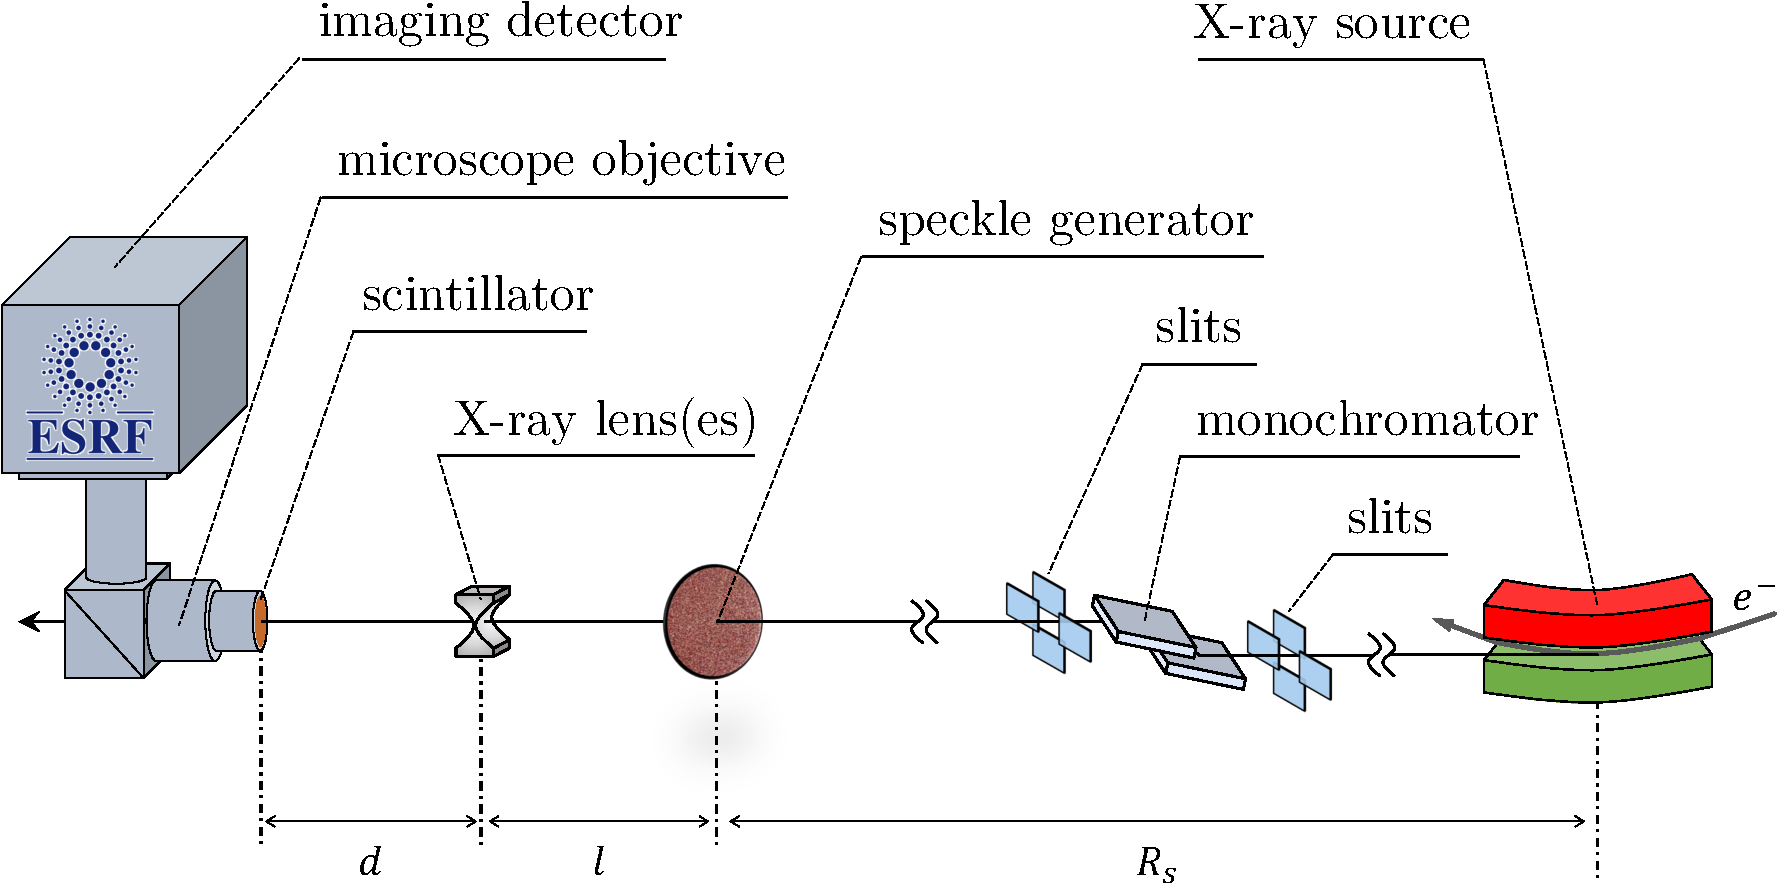
\includegraphics[width=0.7\linewidth]{figures/ch04/BM05.pdf}}
        \caption[Speckle-based imaging experimental setup at the BM05 beamline, ESRF.]{Generic speckle-based imaging experimental setup as originally implemented at the BM05 beamline of the ESRF. \textbf{right to left}: an X-ray source (bending magnet) delivers a beam whose large spectral bandwidth is reduced with a Si(111) double crystal monochromator down to $\Delta \text{E}/\text{E}\approx10^{-4}$. The now monochromatic beam hits the speckle-generator at a distance $R_S$ from the source. The stationary diffuser is composed of several piled up cellulose acetate membrane filters with a mean pore size of 1.2~$\mu$m. The membranes are mounted on a (piezoelectric) nano-positioner transverse translation stage, so that the membranes can be scanned on the $xy-$plane. At a distance $l$ downstream the membrane, the sample is placed and aligned as to the optical axis. Further downstream the probe, at a distance $d$, a scintillator converts the X-rays into visible light. The scintillator is imaged into a 2D imaging sensor , which is coupled with a microscope objective to reach a small pixel size. Such experimental setup, without any structural change, was later on used at the 1-BM (APS) and ID06 (ESRF) beamlines. Conversely to what depicted here, the X-ray source at the ID06 is an undulator and not a bending magnet.} \label{fig:BM05}
\end{figure}

\begin{figure}[t]
        \centering
        {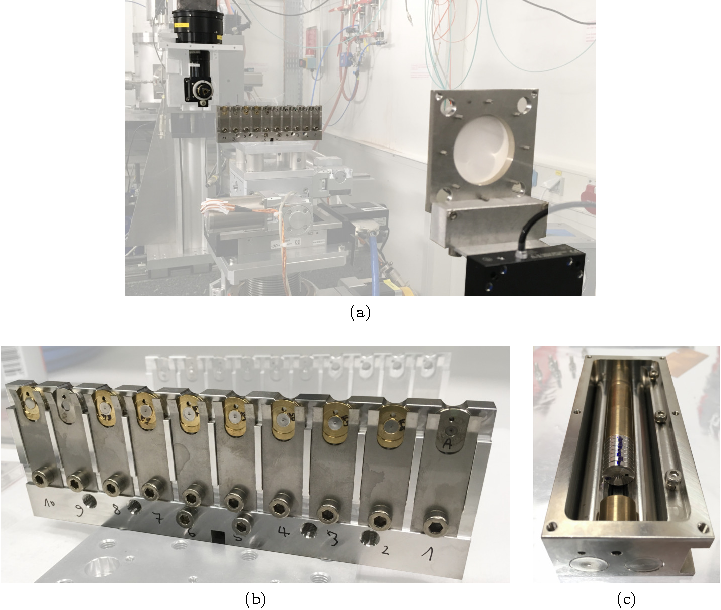
\includegraphics[width=.7\linewidth]{figures/ch04/experimental_setup.pdf}}
        \caption[Experimental setup at the BM05 beamline, ESRF.]{(a) image inside the experimental hutch of the ESRF BM05. The picture highlights the three main components shown schematically in Fig.~\ref{fig:speckle_tracking2}: the detector in the back-plane, the sample-holder specially designed to hold up to 10 lenslets for batch measurements and the speckle-membrane mounted in a (piezoelectric) nano-positioner in the first plane. (b) typical lenslets mounted on the holder designed to provide easy alignment of the lenses in the X-ray beam and ensure repeatable positioning in the lens mount. This holder is designed for single-lens measurement. (c) box required for the  mounting of stacked lenses to be measured together.} \label{fig:experimental_setup}
\end{figure}


X-ray speckle imaging (SBI) can be implemented in several geometries depending on the metrology subject (mirrors, strong focusing mirrors, lenses, stacked lenses) and mode (absolute or differential) - cf. [\cite{Berujon2020a}]. In this section the X-ray (near field) speckle vector tracking (XSVT) in the differential mode, as originally implemented at BM05 and shown in Figs.~\ref{fig:speckle_tracking2}, \ref{fig:BM05} and \ref{fig:experimental_setup} is described.

\subsubsection*{Illumination}

Unlike other wavefront sensing techniques, speckle-based metrology has low requirements on transverse and longitudinal coherence\footnote{Phase-contrast with low-coherence sources has, in fact, been demonstrated [\cite{Cloetens1996, Wilkins1996, Pfeiffer2006, Munro2012}].} as demonstrated by [\cite{Zanette2014,Zdora2015,Wang2016}]. The degree of lateral coherence of the illumination is intimately connected with two important factors: the speckle contrast (cf. Eq.~\ref{eq:visibility}) and the propagation distance where shape and size of the speckle grains are preserved (cf. Eq.~\ref{eq:speckle_goodness}). X-rays with lower transverse coherence will produce speckle with low visibility (smeared out or blurred image) and the numerical process of tracking signals will lose some of its accuracy. For metrology applications, a minimum contrast of 0.1 (Eq.~\ref{eq:visibility}) is expected [\cite{Berujon2020a}] for the algorithms to show an acceptable accuracy. A reduced propagation distance $d$ between the sample and the detector (cf. Fig.~\ref{fig:speckle_tracking2} and \ref{fig:BM05}) arising from a reduced coherence length $\Delta_{\textbf{cl}_\perp}$ (Eq.~\ref{eq:speckle_goodness}) diminishes the angular sensitivity and will impact on the residual height error measurement sensitivity. When selecting an X-ray source, a higher degree of transverse coherence is preferred. Nonetheless, bending magnets\footnote{At BM05, a bending magnet was the X-ray source used in this project until the ESRF-EBS upgrade long shutdown (December 2018). The BM05 bending magnet in place since the opening of the ESRF in 1994 was decommissioned in favour of a much shorter and brighter 2-pole wiggler, installed early 2020. All the data collected at BM05 and presented hereafter were collected before this upgrade.} are readily well suited for  speckle-imaging-based metrology since their beam usually offer a the necessary minimum transverse coherence  \footnote{As of the writing of this thesis, the beamlines the routinely offer X-ray lenses metrology with speckle-based-imaging are the BM05 (ESRF) [\cite{Berujon2020a}], 1-BM (APS) [\cite{Qiao2020}] and B16 (DLS) [\cite{Sawhney2013}].}. 

Choosing the experiment energy\footnote{The energy chosen for most metrology experiments was $\text{E}=17~$keV with $\Delta \text{E}/\text{E}\approx10^{-4}$ by using a Si(111) DCM. This energy was originally set at the BM05 due to the source higher flux at this energy (the critical storage ring energy was around 19 keV) and the good compromise between absorption and sensitivity such working wavelength offer. Later, this same energy was also adopted for experiments at other beamlines in order to facilitate direct comparison during the data-analysis.} for X-ray lens metrology is about reaching a compromise between several competing constraints. For a fixed distance $d$, the energy should be high enough so that the speckle grains being transmitted through the lens geometric aperture are not excessively deformed by focusing at the detection plane - the higher the energy, the longer the focal length of a X-ray lens is (cf. Eq.~\ref{eq:CRL_classic}) - on the other hand, a lower energy gives larger refraction angles, which increases the sensitivity of the experimental technique. Excessive deformation of the transmitted speckle field, however, causes the tracking to fail in delivering credible results. Higher energy is also beneficial when considering the limit to the distance $d$ imposed by Eq.~\ref{eq:speckle_goodness}. On the other hand, increasing the energy decreases the coherent fraction of the emitted beam, which in turn reduces the speckle visibility\footnote{Slitting down the beam and increasing the propagation distance from the source to the speckle-membrane ($R_s$ in Fig.~\ref{fig:BM05}) both help to increase the coherence length at the expense of photon flux - cf. van-Cittert-Zernike theorem in [\cite[\textit{§4.4.4}]{Mandel1995}] or the applicability to SR in [\cite[\textit{§4}]{Geloni2008}].}. Lastly, the source spectrum (Fig.~\ref{fig:emission}) has also to be considered, as a higher photon flux allows for shorter acquisition time, meaning that experiments require less time and possible instabilities (vibrations, long time drifts and other external perturbations) have a lower impact on the acquired data. Requirements on the illumination monochromaticity are not stringent for SBI, but the metrology of X-ray lenses requires narrow bandwidths as these optics suffer from intrinsic strong aberrations. In order to secure a good lateral resolution, a Si(111) double crystal monochromator (DCM)\footnote{Yet, an experimental comparison between the metrology data obtained with a Si(111) DCM with $\Delta \text{E}/\text{E}\approx10^{-4}$ and a multi-layer monochromator with $\Delta \text{E}/\text{E}\approx10^{-2}$ showed very good agreement between both data-sets [\cite[\textit{\S3.3.3}]{Berujon2020a}].} is usually used to bring down the bandwidth to $\Delta \text{E}/\text{E}\approx10^{-4}$.

\subsubsection*{Speckle membrane}

Unlike other wavefront techniques that require specially tailored optics that may need laborious alignment procedures such as reference phase-objects (Siemens star) or gratings, SBI requires a transmission element with transversely randomly distributed small features. The random optical path differences generated by these objects or grains must be capable of producing speckle-grains that covers a few pixels (<10 pixels) at the detector with visibility of $ v>0.1$ [\cite[\textit{\S2.3}]{Berujon2020a}]. Early experiments were done by stacking commercially available abrasive paper (sandpaper) until the desired speckle pattern was obtained\footnote{More recent guidelines helping to choose the appropriate sandpaper grain size (grit) for an experimental setup were published by [\cite{Tian2020}].} [\cite{Morgan2012, Wang2016}]. The choice of a modulator depends on the experiment energy and the detector, but often, static granular materials, sandpaper of diverse grits and filters with micrometric pore-sizes cen be used\footnote{Experiments shown here used a stack of cellulose acetate membrane filters with a mean pore size of 1.2~$\mu$m used as the stationary diffuser.}. Low transmission, poor time stability and/or the presence of strong diffraction are characteristics that should be avoided when choosing a speckle generator. Due to the random nature of the wavefront (static) modulation, the membrane does not require any precise alignment with  the beam. 

XSVT is a a scanning technique and customary\footnote{More details in data acquisition are provided by \S\ref{sec:data}~-~\textit{\nameref{sec:data}}.} $N$ reference images are taken at $N$ different transverse positions of the speckle generator with respect to the optical axis. The sample is put into the beam and another set of $N$ images are taken with the speckle generator located at the exact previous $N$ positions - cf. orange arrows in Fig.~\ref{fig:speckle_tracking2}. The reproducibility of the speckle generator transverse positions is of key importance as the difference in the speckle grain positions from reference to sample image is attributed to the modulation of the beam. To make sure that during the collection of the $j^\text{th}~(j\in[1,2,...,N])$ pair of images the position of the speckle generator is repeated with a precision as good as a fraction of effective pixel size, the modulator is mounted on a (piezoelectric) nano-positioner with a travel range of at a few hundreds micrometers.

\subsubsection*{Sample}

X-ray speckle vectorial tracking is a very attractive technique as it can measure weak-focusing optics as well as very strong focusing systems with minor modifications of the setup - cf. [\cite{Berujon2020a}] for some examples. Typically, two types of optical elements are today routinely measured at the ESRF: individual lenses and moderately focusing CRLs. Figure~\ref{fig:experimental_setup}(b) and (c) shows typical lenses in their holder. Single lenses are mounted in an in-house-designed holder conceived to hold up to 10 lenslets next to each other, allowing serial measurements and minimising manual intervention to change samples. Stacked lenses are measured in typical casings. The lens holder has to be mounted on a motorised support that can move transversely to the beam ($xy-$plane) and has yaw, pitch, and roll rotations\footnote{Yaw was defined in our case as the rotation around the $z-$axis, the pitch is around the $y-$axis and roll, the $x-$axis.} to compensate for the residual phase errors generated from misalignments - cf. \S\ref{sec:misalignments}~-~\textit{\nameref{sec:misalignments}}. 

\subsubsection*{Detection}

Although subpixel resolution for XSVT has been recently reported [\cite{Qiao2020b}], generally, the lateral resolution of the 2D surface maps obtained with XSVT is limited to the detector effective pixel size. This makes the use of a 2D high-resolution imaging detectors common for for speckle-based imaging. In real-space imaging with X-rays, since high resolution over a large field of view is usually wished, it is common to use indirect detection. Converting X-rays into visible-light and subsequently imaging it onto a pixelated detector allows one to access to smaller pixel sizes thanks to the use of magnifying optics and small pixel sensors designed for visible-light detection.

A typical detection system\footnote{The detection systems use at the ESRF are composed of a 10~$\mu$m thick LSO:Tb scintillator that is imaged onto an sCMOS PCO Edge 4.2 or a FReLoN E2V CCD camera (2048 $\times$ 2048 pixels), coupled with a 10$\times$ magnification microscope objective to reach a theoretical pixel size of about $\sim0.62\times0.62~\mu$m$^2$. At the APS, the scintillator used was a 100~$\mu$m thick LuAG:Ce imaged into an Andor Neo sCMOS camera with 2560 $\times$ 2180 pixels also with a 10$\times$ magnification resulting in a pixel size of $\sim0.65\times0.65~\mu$m$^2$.} is composed of three main parts: \textit{i}-) the scintillator, which is responsible for converting the X-rays into visible light. Its choice is a compromise between the yield in converting X-ray photons in visible photons and image sharpness: a thin scintillator will generally result in a sharper image, but at a cost of a reduced photon flux, while a thicker one will generate more light, but due to scattering in the bulk material, a less sharp image will be available; \textit{ii}-) the transport optics that magnifies and images the scintillator onto the sensor plane, but also may introduce aberrations to the system, but can be calibrated with the XSVT technique - cf. [\cite[\textit{\S2.2}]{Berujon2020a}]; and \textit{iii}-) the imaging sensor, which ideally should be a low-noise 2D pixelated sensor with fast read-out. The final effective pixel size is a convolution of the contributions from the choice of scintillator, magnification and point spread function of the transport optics and the imaging device.

\begin{figure}[t]
        \centering
        {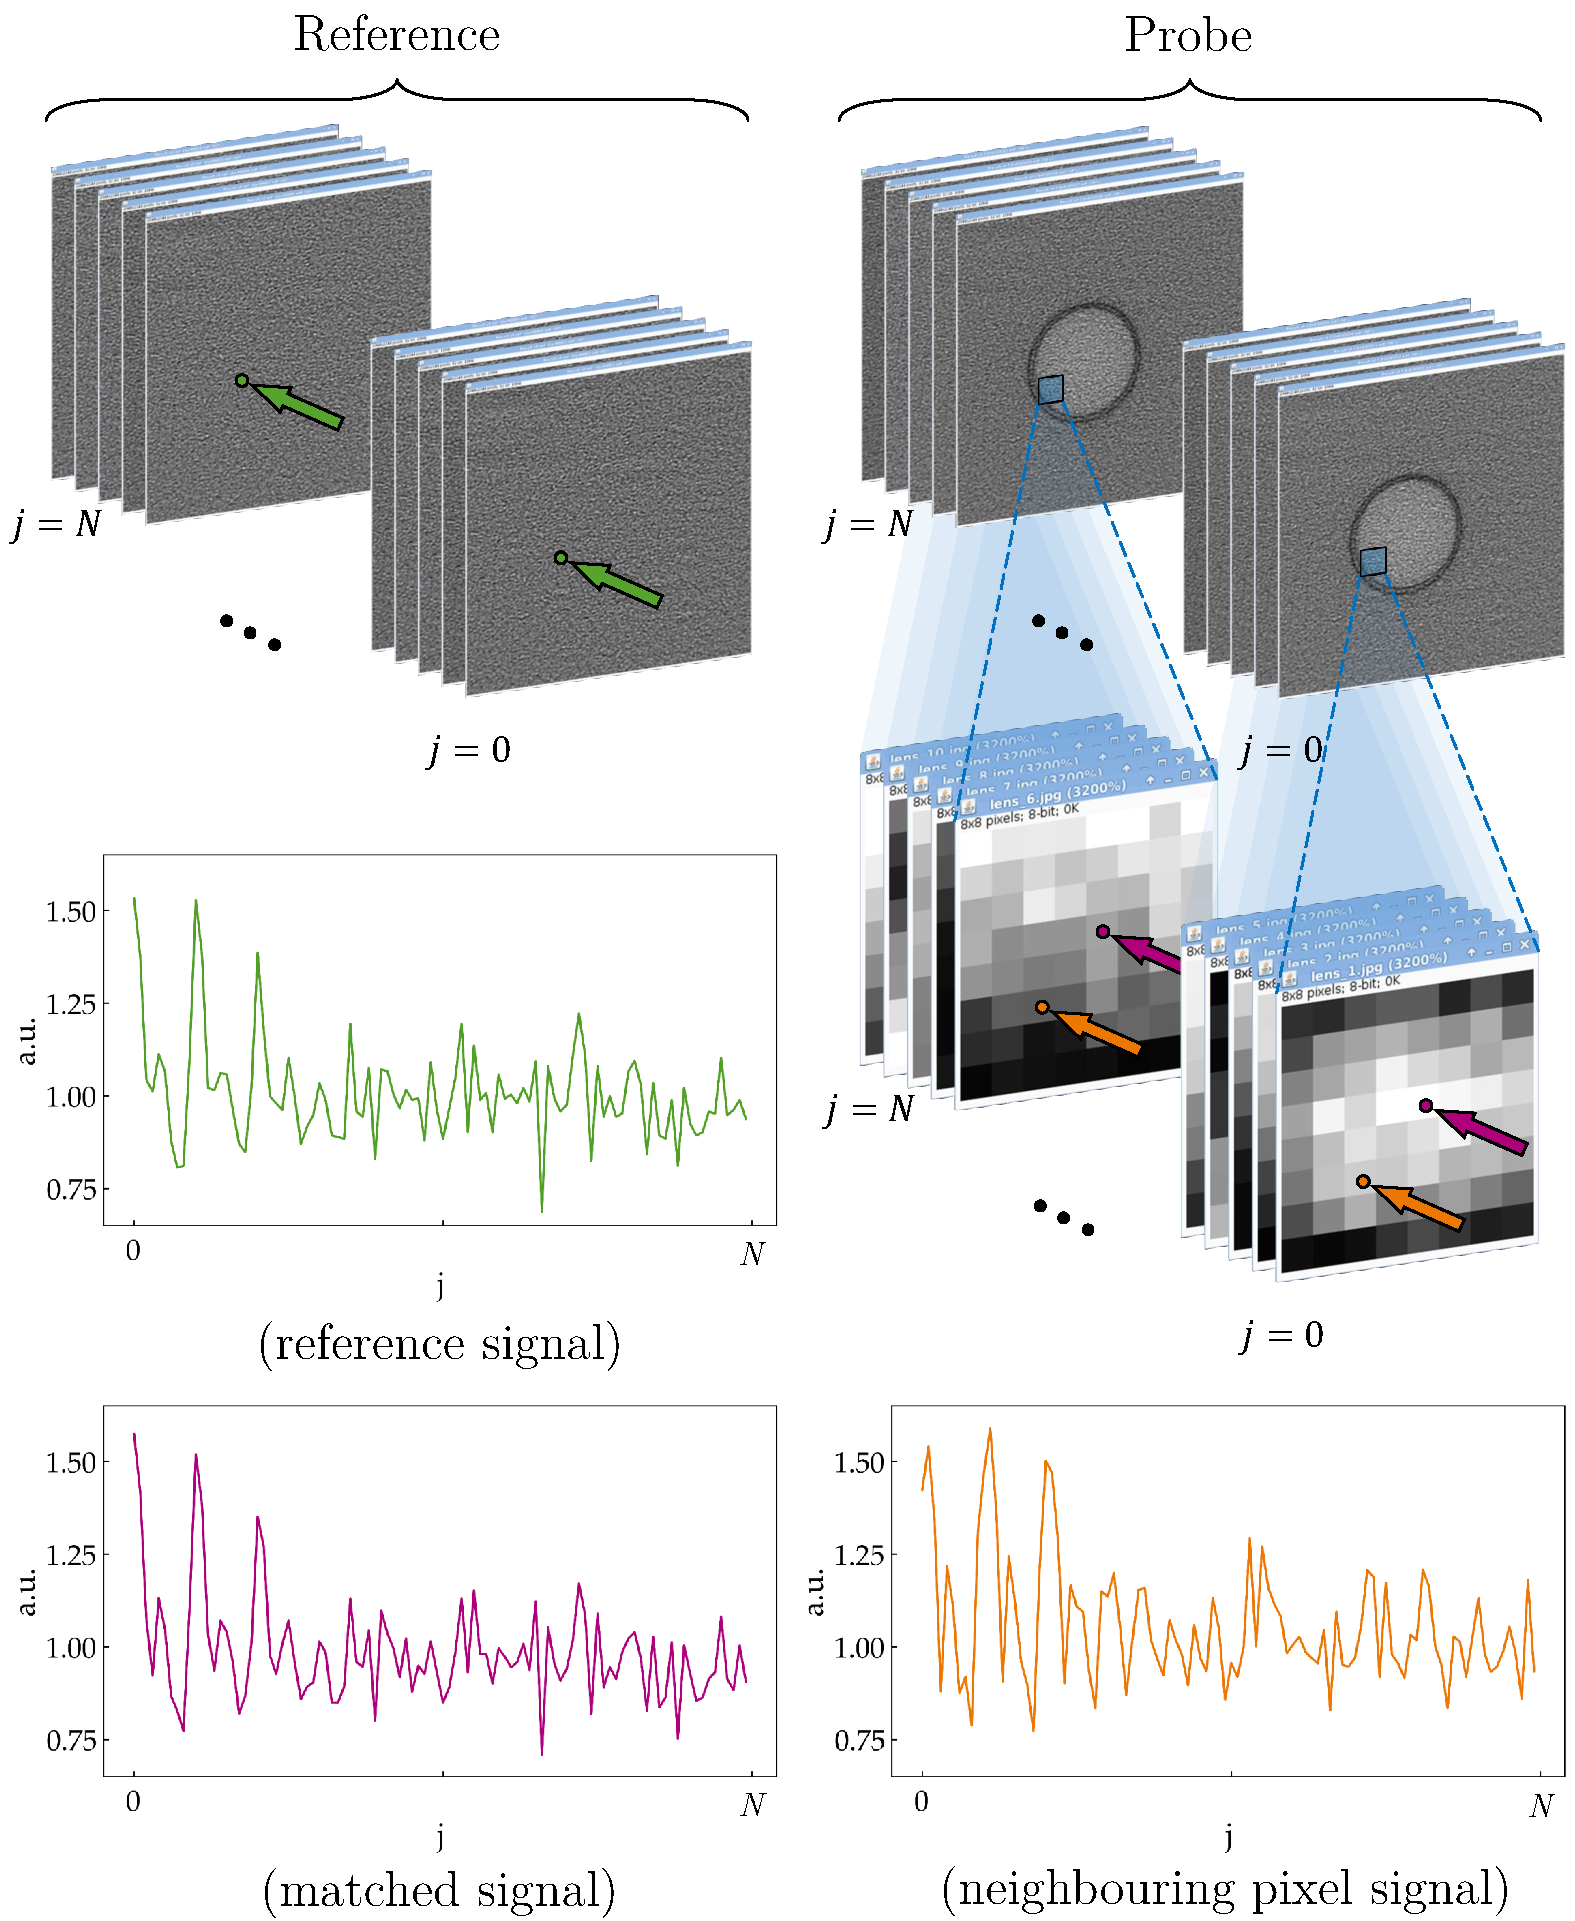
\includegraphics[width=.7\linewidth]{figures/ch04/speckle_data.pdf}}
        \caption[X-ray (near field) speckle vector tracking (XSVT)]{X-ray (near field) speckle vector tracking (XSVT). In the differential mode, two data-sets are taken: the reference and the one with the imaged sample. Each of the $j^\text{th}$ image pair of the data-set is taken at a different transverse scan position of the speckle-generator across the X-ray beam. However, for a particular $j^\text{th}$ image-pair
        (reference and probe) the exact same diffuser position must be maintained. A reference intensity vector $I_{\text{reference}}(x_l,y_m,j)$ (green) is searched in the smaple stack,in a ROI centred around $(x_l,y_m,j)$, where $I_{\text{probe}}(x_{l+\Delta l},y_{m+\Delta m},j)$ vectors are probed for a matching value. The purple signal is a well matched signal, while the orange signal shows the neighbouring-pixel intensity vector $I_{\text{probe}}(x_{l-2},y_{m-2},j)$.}\label{fig:data_tracking}
\end{figure}

\newpage
\newpage
%-------------------------------------------------------------------------
%-------------------------------------------------------------------------
\subsection{Data acquisition, processing and analysis}\label{sec:data}
%-------------------------------------------------------------------------
%-------------------------------------------------------------------------

\subsubsection*{Data acquisition \& analysis}

The first implementations of X-ray speckle-tracking (XST) for metrology consisted of acquiring solely two images: the reference- and the sample-image with the same speckle pattern (cf. Fig.~\ref{fig:speckle_tracking}). The algorithms used to match the patterns in both images relied in setting in the reference image a small window around a pixel of interest $w_\text{reference}(x_l,y_m)$ and searching for it (possibly distorted) in a larger window in the sample image: $w_\text{probe}(x_l,y_m)$. The reference window is rastered through the whole sample image ($L\times M$ pixels) to reconstruct two 2D displacement maps (horizontal and vertical) with lateral resolution limited to the speckle-grain size. In order to improve the limited resolution of XST, XSVT relies on transversely scanning\footnote{The nature of the scan is not particularly relevant for the data analysis in this particular metrology mode.} the speckle-generator across the X-ray beam and taking images at the $N$ different points of the scan. Once the reference data-set is taken, the sample is inserted in the beam and the scan is repeated at the exact same diffuser position. Each data set (reference and probe) contains $N_{L\times M}$ images where the $j^\text{th}~(j\in[1,2,...,N])$ image in each stack indicates the same transverse coordinates of the scatterer scan - cf. Fig.~\ref{fig:data_tracking}. For a sufficiently large $N$, a vector is obtained by sampling each $j^\text{th}$ image of the reference data-set around a pixel coordinate $(x_l,y_m)$ with $l\in[1,2,...,L]$ and $m\in[1,2,...,M]$. This reference signal $I_{\text{reference}}(x_l,y_m,j)$ is shown in green in Fig.~\ref{fig:data_tracking}. A ROI centred in $(x_l,y_m)$ is set in the sample data-set and for each pixel coordinate within this ROI, that is $(x_{l+\Delta l},y_{m+\Delta m})$, a corresponding intensity vector is obtained: $I_{\text{probe}}(x_{l+\Delta l},y_{m+\Delta m},j)$ - cf. magenta and orange signals in Fig.~\ref{fig:data_tracking}. The $I_{\text{reference}}(x_l,y_m,j)$ vector is compared\footnote{Which can be either using a cross-correlation peak calculation [\cite{Berujon2012, Morgan2012}], a least-square-minimisation [\cite{Zanette2014, Zdora2017}] or an Euclidean-distance minimisation of the wavelet-transform of the reference- and probe- vectors [\cite{Qiao2020b}].  In this work the cross-correlation peak calculation is the preferred method for speckle-vector tracking [\cite{Berujon2012, Morgan2012}].} individually to each of the $I_{\text{probe}}(x_{l+\Delta l},y_{m+\Delta m},j)$ vectors. Fig.~\ref{fig:cross-correlation-map} shows the normalised cross-correlation values for a particular lens, which are used to evaluate the convergence of the tracking method. By repeating this procedure for all $L\times M$ pixels, it is possible to obtain two 2D displacement maps (vertical and horizontal) with lateral resolution down to the $\sim$~effective-pixel-size of the detector at the expense of an increased data-collection and data-processing time[\cite{Berujon2016,Berujon2020}].

\begin{figure}[t]
        \centering
        {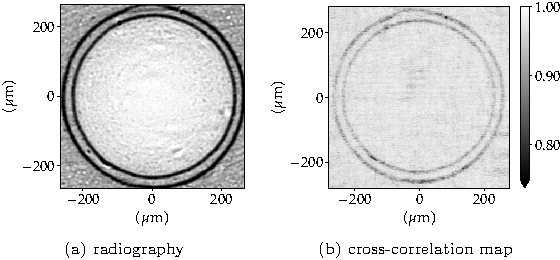
\includegraphics[width=.5\linewidth]{figures/ch04b/radio_corr_map.pdf}}
        \caption[Normalised cross-correlation map]{(a) radiography of a 2D-Beryllium lens with $R=50~\mu$m measured at 17~keV with $d=800$~mm and pixel size $\Delta_\text{pixel}= 0.63~\mu$m. The different penetration depths of the parabolic profiles cause the reduction of the geometric aperture, evidenced by the two concentric rings. (b) the normalised cross-correlation peak for the vector tracking algorithm. Regions with darker colours have lower correlation peaks.}\label{fig:cross-correlation-map}
\end{figure}

\begin{figure}[t]
        \centering
        {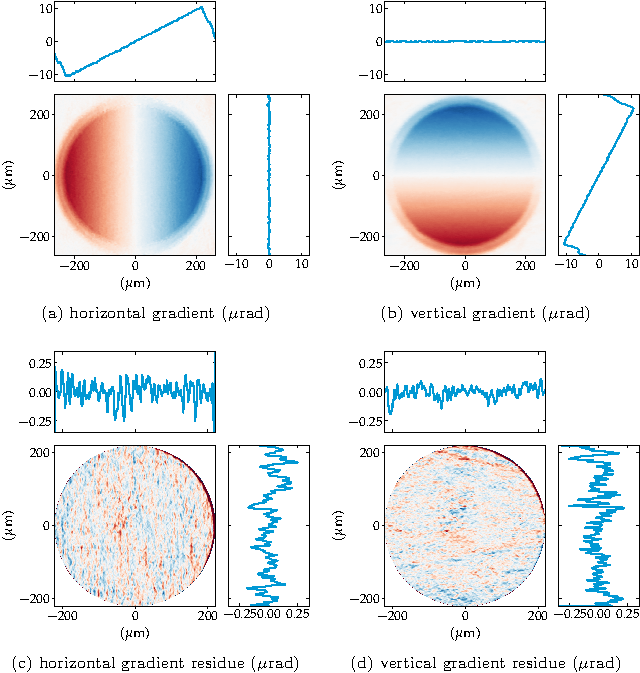
\includegraphics[width=.6\linewidth]{figures/ch04b/gradients.pdf}}
        \caption[Recovered phase gradient and residues]{(a) horizontal and (c) vertical phase gradients for the 2D-Beryllium lens with $R=50~\mu$m measured at 17~keV with $d=800$~mm and a pixel size $\Delta_\text{pixel}= 0.63~\mu$m - cf. Fig.~\ref{fig:cross-correlation-map}.}\label{fig:gradients}
\end{figure}

\begin{figure}[t]
        \centering
        {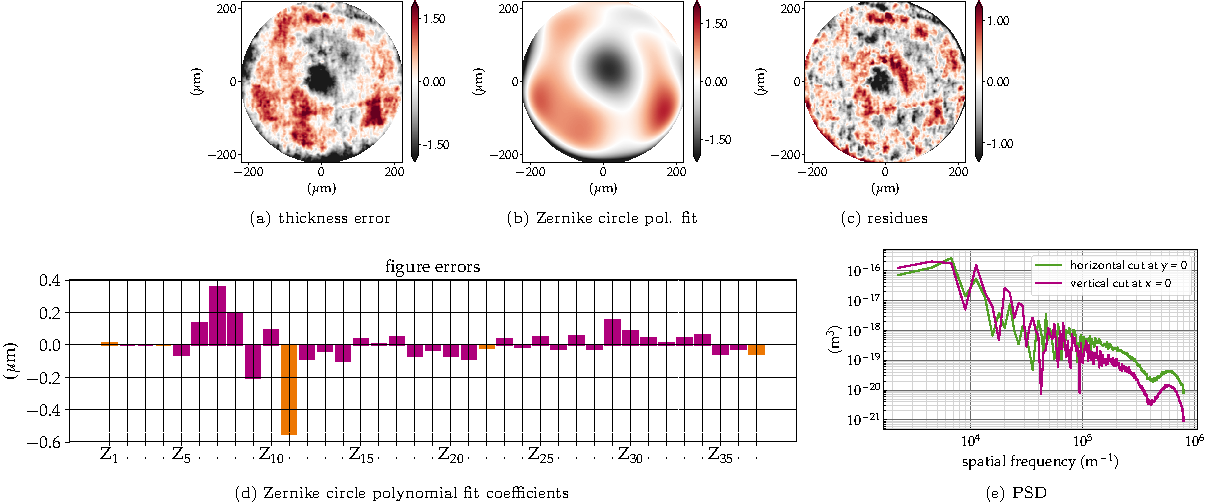
\includegraphics[width=1\linewidth]{figures/ch04b/recovered_thickness.pdf}}
        \caption[Recovered figure errors in projection approximation]{(a) Recovered figure errors in projection approximation of a 2D-Beryllium lens with $R=50~\mu$m measured at 17~keV with $d=800$~mm and pixel size $\Delta_\text{pixel}= 0.63~\mu$m, (b) Zernike circle polynomial fit of the figure errors and (c) the residues from the fit. The coefficients of the fit are shown in (d). (e) Power spectrum density of the horizontal and vertical cuts passing through the centre of the lens.}\label{fig:recovered_thickness}
\end{figure}

\subsubsection*{Surface reconstruction \& analysis}

The phase gradients $\nabla\phi(x,y)$ can be obtained from the two displacement maps by multiplying them by the wavenumber $k$ and dividing the product by the distance between the sample and detector ($d$) - cf. Eq.~\ref{eq:wavefront_gradient}. An example of the horizontal and vertical gradient for a 2D-Beryllium lens with $R=50~\mu$m measured at 17~keV with $d=800$~mm and pixel size $\Delta_\text{pixel}= 0.63~\mu$m is shown in Fig.~\ref{fig:gradients}(a)-(b) where the mismatch between front- and back- focusing surfaces is obvious - cf. Fig.~\ref{fig:cross-correlation-map}. An ideal lens has phase gradients with linear dependencies on the focusing direction. From Eq.~\ref{eq:aux_funcs_transb} and Eq.~\ref{eq:ProjecThick}: 
\begin{align}
    \nabla\phi(x,y) & = \Bigg(\frac{\partial \phi(x,y)}{\partial x},\frac{\partial \phi(x,y)}{\partial y}  \Bigg) = -2k\delta\Bigg(\frac{x}{R_x},\frac{y}{R_y}\Bigg),
\end{align}{}
which is a linear function with the slope of the linear phase-gradient in the focusing direction inversely proportional to the radius of curvature of the X-ray lens. This information  can be experimentally retrieved with the knowledge of the X-ray energy used and the lens material (refraction index decrements). The phase gradient residues (or errors) are accessible by removing a linear fit from the gradients, which is shown in Fig.~\ref{fig:gradients}(c)-(d). In order to recover the thickness profile in projection approximation from the phase gradient (or from the residual phase gradient), the main step is the numerical 2D integration\footnote{More on numerical integration of gradient fields in [\cite{Huang2015}] and [\cite{Agrawal2006}].} of the differential fields, which is done using either the Frankot-Chelappa method [\cite{Frankot1988}] or the Harker-O'Leary method ($\text{grad2surf}$) [\cite{Harker2015}]. 

The profile resulting from the 2D integration of the (residual) phase gradients can be converted into thickness in projection approximation by (cf. Eq.~\ref{eq:aux_funcs_transb}):
\begin{align}\label{eq:recovered_thickness}
     \Delta_z(x,y)&=-\frac{\phi(x,y)}{k\delta}.
\end{align}{}
Eq.~\ref{eq:recovered_thickness} is based on the assumption that the X-ray lens has a refraction index decrement $\delta$ with no variations in $(x,y,z)$. Eq.~\ref{eq:recovered_thickness} also justifies the use of a monochromator in the experimental setup (cf. Fig.~\ref{fig:BM05}) since $\delta$ has an important energy dependency. The figure errors from a lens can be obtained by two approaches: \textit{i}-) by first integrating the phase gradients, then fit and remove from the resulting surface either a cylinder with a parabolic section or a paraboloid of revolution depending on whether the lens is a 1D or 2D focusing element. The treatment shown in Eq.~\ref{eq:recovered_thickness} is applied to this residual phase; or by \textit{ii}-)directly integrating the residual phase gradients and application of Eq.~\ref{eq:recovered_thickness} to the integrated field. The residual thickness in projection approximation for the previous lens is shown in Fig.~\ref{fig:recovered_thickness}(a). Valuable information such as the RMS value of the figure errors; the decomposition of the wavefront into orthonormal polynomials (cf. \S\ref{sec:orthonormal_polynomials}~-~\textit{\nameref{sec:orthonormal_polynomials}}) for the systematic study of the optical imperfections; and the power spectral density (PSD) of horizontal- and vertical- profile cuts showing the spatial frequency distribution of the optical errors can all be obtained from the residual thickness profile as shown in Fig.~\ref{fig:recovered_thickness}. The recovered thickness profile in Fig.~\ref{fig:recovered_thickness}(a) can be later used as a $\Delta_z(x,y)$ map in Eq.~\ref{eq:transmission_operator} to simulate the effects of optical imperfections in X-ray lenses as discussed in \S\ref{sec:metrology_data}~-~\textit{\nameref{sec:metrology_data}} from \S\ref{sec:other_sources}~-~\textit{\nameref{sec:other_sources}}. 

\subsubsection*{Measurement sensitivity}

Finally, some considerations on the measurement sensitivity. Supposing an ideal detection system with effective pixel size $\Delta_\text{pixel}$, the minimum measurable deflection angle is:
\begin{align}\label{eq:alpha_min}
    \alpha_\text{min}=\eta\frac{\Delta_\text{pixel}}{d},
\end{align}
where $\eta$ is a factor accounting for the ability of the algorithm to track a displacement vector with subpixel accuracy. Consider that the probe can be laterally sampled with the detector spatial resolution $\Delta_\text{pixel}$ as shown in Fig.~\ref{fig:sensitivity}(a). Each projected pixel will have a mean height value and the minimum detectable height difference between two adjacent pixels is $\Delta{z_{\text{min}}}$. The angle $\alpha_\text{min}$ can be attributed to refraction caused by the local slope $\vartheta$ between two adjacent projected pixel - cf. Fig.~\ref{fig:sensitivity}(b). A ray that is parallel to the optical axis will intercept this local slope at an angle $\theta_1=\vartheta$ and will be refracted with an angle $\theta_2=\vartheta+\alpha_\text{min}$. With the law of refraction (Eq.~\ref{eq:refraction}) it is possible to estimate\footnote{From Fig.~\ref{eq:XSVT_resolution}(a) one obtains: $\tan(\vartheta)=\cfrac{\Delta{z_{\text{min}}}}{\Delta_\text{pixel}}$. Using $n_1=1$, $n_2=1-\delta$, $\theta_1=\vartheta$ and  $\theta_2=\vartheta+\alpha_\text{min}$ in the law of refraction: $\sin(\vartheta)=(1-\delta)\sin(\vartheta+\alpha_\text{min})$. Writing $\sin(\vartheta+\alpha_\text{min})=\sin(\vartheta)\cos(\alpha_\text{min})+\sin(\alpha_\text{min})\cos(\vartheta)$ and collecting terms, one obtains Eq.~\ref{eq:XSVT_resolution}. Similar reasoning can be applied to a two-refraction model giving very similar numerical results.} the longitudinal sensitivity of the XSVT as\footnote{It is also possible to derive an approximate expression by using physical-optics arguments. The accumulated phase of a wave transversing a material with thickness $\Delta_z$ and index of refraction $n=1-\delta+i\cdot\beta$ is $\phi(x,y)=k\delta\Delta_z$ as shown in Eq.~\ref{eq:aux_funcs_transb}. The gradient of this phase is: $\nabla \phi(x,y)=\Bigg(k\delta\cfrac{\partial}{\partial x}\Delta_z; k\delta\cfrac{\partial}{\partial y}\Delta_z\Bigg)$. The partial derivatives (local slopes) can be calculated as: $\cfrac{\partial}{\partial x}\Delta_z = \cfrac{\partial}{\partial y}\Delta_z = \cfrac{\Delta_z}{ \Delta_\text{pixel}}$ as a first approximation for a square pixel. With the help of Eq.~\ref{eq:wavefront_gradient} and Eq.~\ref{eq:alpha_min} one arrives at: $\Delta{z_{\text{min}}}=\Delta_\text{pixel}\cdot\cfrac{\alpha_\text{min}}{\delta}$.}: 
% \begin{align}\label{eq:XSVT_resolution}
% \Delta{z_{\text{min}}}=\eta\Delta_\text{pixel}\cdot\frac{\sin(\alpha_\text{min})}{\cfrac{1}{1-\delta}-\cos(\alpha_\text{min})}.
% \end{align}
\begin{align}\label{eq:XSVT_resolution}
\Delta{z_{\text{min}}}=\Delta_\text{pixel}\cdot\frac{\sin(\alpha_\text{min})}{\cfrac{1}{1-\delta}-\cos(\alpha_\text{min})}.
\end{align}
Figure~\ref{fig:sensitivity_2} shows the XSVT longitudinal sensitivity ($\Delta{z_{\text{min}}}$) based on Eq.~\ref{eq:XSVT_resolution} for four common used materials for refractive optics manufacturing. From Eq.~\ref{eq:XSVT_resolution}, it clear that longitudinal resolution of the XSVT technique depends on several factors: distance between speckle-generator and detector $d$; material and experiment energy expressed as index of refraction decrement $\delta$; and the the effective pixel size $\Delta_\text{pixel}$, which is directly impacted by the PSF of the transport optics of the imaging system. Other factors that contribute to the reduction in lateral resolution (increase $\eta$): \textit{i}-) the thickness of the scintillator used (blurring from thicker materials), \textit{ii}-) temporal beam-instabilities as they may reduce the apparent transverse coherence if the integration time of the detector is longer than the instabilities period; \textit{iii}-) vibrations of the sample holder with amplitudes larger than half of the pixel size and faster than the acquisition time. A low reproducibility of the speckle-generator membrane positioning in the X-ray beam and decreases the sensitivity as any change in speckle position in a differential measurement, regardless of its origin, is attributed to the sample modulation of the wavefront markers.  

\begin{figure}[t]
        \centering
        {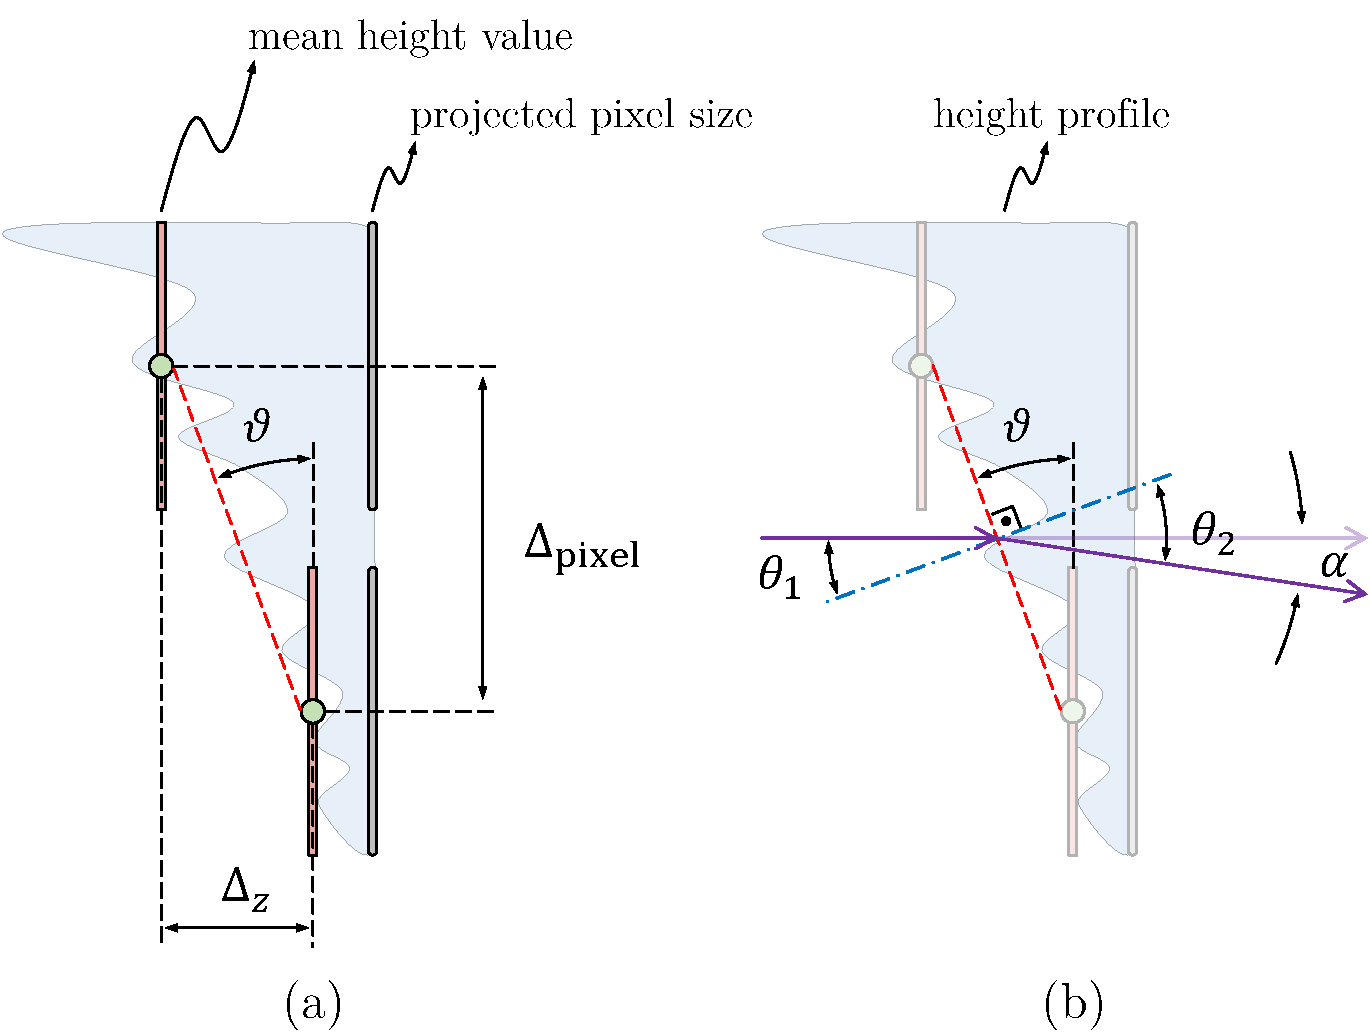
\includegraphics[width=0.5\linewidth]{figures/ch04b/sensitivity.pdf}}
        \caption[XSVT sensitivity calculation sketch]{Sketch for aiding the calculation of the XSVT longitudinal sensitivity. The lateral resolution to which the probe is sampled generates a local slope between adjacent pixels (red dashed line with inclination given by $\vartheta$). A beam parallel to the optical axis (purple) hits the sample is refracted with an angle $\theta_2$.}\label{fig:sensitivity}
\end{figure}

Equation~\ref{eq:XSVT_resolution} is a geometric approximation of the problem and does not take into account propagation of uncertainties associated with the different components in the experiment, template-matching accuracy of the tracking routines nor numerical errors associated with the wavefront reconstruction as described by [\cite{Fried1977, Southwell1980}]. Those can be globally estimated by applying the XSVT data analysis routine to two different data-sets taken under the exact same experimental conditions. The two 2D deflection angle maps allow to obtain the angular sensitivity lower threshold and to estimate $\eta$ under the conditions imposed by the experimental setup. Those maps can be integrated to obtain the phase noise level (see Eq.~\ref{eq:wavefront_gradient}) and an associated thickness can by estimated by using Eq.~\ref{eq:recovered_thickness}. Applying the same reasoning to a single set of references used as both the reference- and sample-data sets instead, allows to calculate a fundamental data-processing limit.


%-------------------------------------------------------------------------
%-------------------------------------------------------------------------
\section{X-ray lenses metrology}\label{sec:metrology}
%-------------------------------------------------------------------------
%-------------------------------------------------------------------------

Since early 2017, metrology of individual X-ray lenses has been systematically done at the ESRF. Measurements have been applied to quality control of commercially acquired X-ray lenses either for assessing the optical quality of already purchased lenses and for verifying if newly-purchased lenses meet specifications. The metrology profiles extracted from such measurements have been used in X-ray beamline simulations\footnote{Simulations using optical metrology of X-ray lenses have been reported in [\cite{Chubar2020}].} [\cite{Celestre2020}]. More recently, metrology started to be used in order to aid manufacturing of X-ray lenses produced in-house\footnote{See [\cite{Celestre2020c}].} or as a co-development with commercial partners as it allows to understand the relation between production parameters and their effects on the lens profile.

%-------------------------------------------------------------------------
%-------------------------------------------------------------------------
\subsection{Single lens measurements}\label{sec:single_lens}
%-------------------------------------------------------------------------
%-------------------------------------------------------------------------

Tables~\ref{tab:CDn} and \ref{tab:CDo} show a compilation of radii, figure errors and useful geometric aperture for two sets of ten 2D-Beryllium lenses with nominal radius $R=50~\mu\text{m}$ and geometric aperture $A_{\diameter}=440~\mu\text{m}$ measured individually and as stacks. These are the lenslets used for in the optical simulations shown in \S\ref{sec:effect_optical_imperfections}~-~\textit{\nameref{sec:effect_optical_imperfections}} and \S\ref{sec:corrections}~-~\textit{\nameref{sec:corrections}}. The figure errors are divided in full profile, polynomial fit (low frequency - LF) and residues from the fit (high-frequency - HF). For the particular case of the 2D-Beryllium lenses, Zernike circle polynomials until the 37$^\text{th}$ order (3$^\text{rd}$ order spherical aberration) were used. In the context of this work, the low-frequencies (LF) span from $\sim500~\mu$m or $2\times10^{3}~\text{m}^{-1}$ (geometrical aperture of a lenslet) to $\sim50~\mu$m or $2\times10^{4}~\text{m}^{-1}$, while the mid- and high-frequencies span from $\sim50~\mu$m or $2\times10^{4}~\text{m}^{-1}$ to $\sim0.5~\mu$m or $2\times10^{6}~\text{m}^{-1}$, which is obtained from the Nyquist frequency\footnote{Nyquist frequency is defined as one over twice the effective pixel size $\Delta_\text{pixel}=0.65~\mu$m.} of the measured data.

Individually measured lenses can be artificially stacked to study the effects of pilling up lenses and to be later compared to the measurement of stacked lenses. This artificial stacking can be done by propagating a plane wave through the CRL and extracting any developed quadratic phase term at the exit pupil - see Fig.~\ref{fig:accumulated_extraction}. The phase can be readily converted into a thickness profile in projection approximation with the aid of Eq.~\ref{eq:aux_funcs_transb}. The accumulated\footnote{The progressive increase of figure errors for the full-, fit- and residual- profiles is shown in Fig.~\ref{fig:stacking_errors} from \S\ref{sec:stacking}~-~\textit{\nameref{sec:stacking}}} profiles for the stacks 1 and 2 are shown in Figs.~\ref{fig:accumulated_profile_1} and~\ref{fig:accumulated_profile_2} and compiled in Tables~\ref{tab:CDn} and \ref{tab:CDo}.  

%-------------------------------------------------------------------------
%-------------------------------------------------------------------------
\subsection{Stacked lenses measurements}\label{sec:lens_stack}
%-------------------------------------------------------------------------
%-------------------------------------------------------------------------

Being able to measure stacked lenses is also of high interest as it allows not only to predict the performance of such focusing compound element in conditions relatively similar to their employment in beamlines, but also enables to design optical corrections for an aberrated system [\cite{Seiboth2017, Seiboth2020}]. The values for radii, figure errors and useful geometric aperture for the two stacks used in this work are shown in Tables~\ref{tab:CDn} and \ref{tab:CDo} and Figs.~\ref{fig:CDn} and \ref{fig:CDo}. The stacks, composed of the lenses described in \S\ref{sec:single_lens}~-~\textit{\nameref{sec:single_lens}} can be compared with the artificially accumulated profiles as shown in Figs.~\ref{fig:accumulated_profile_1} and~\ref{fig:accumulated_profile_2}, which shows reasonable qualitative agreement - improving the agreement between the two types of measurements is important as it allows the prediction of performance and correction of a CRL composed of an arbitrary set of already measured and catalogued lenses. $\blacksquare$

\begin{figure}[t]
    \centering
    {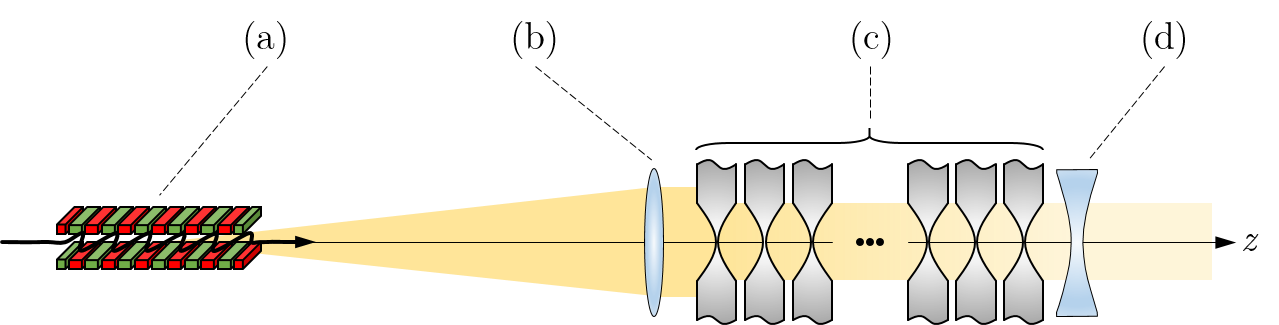
\includegraphics[width=.7\linewidth]{figures/ch04b/recovered_phase.png}}
    \caption[Optical layout used for artificially stacking lenses]{Optical setup used for artificially stacking lenses and calculating the phase errors. The electron-beam parameters are the ones from the ESRF-EBS upgrade [\cite{orangebook}]. The illumination is filament electron beam passing through a (a) CPMU18 undulator with 111 magnetic periods with $\Lambda=18$~mm magnetic period and magnetic field $B=0.9863~$T - cf. \S\ref{sec:brilliance}~-~\textit{\nameref{sec:brilliance}}. An (b) ideal parabolic phase element with radius of curvature $R=-60~$m is placed 60~m downstream the radiation source to give the illumination a near-plane phase - cf. Eq.~\ref{eq:planewave}. The stacked X-ray lenses are placed immediately downstrem. They follow the model described by Eq.~\ref{eq:TE_CRL_MS_ERR}, that is, the CRL multi-slicing with figure errors added. Any changes to the wave-field after (c) can be directly attributed to the the model under study. An (d) ideal parabolic phase element with radius of curvature matching the developed quadratic term is then added and the residues (phase errors) can be extracted.}
    \label{fig:accumulated_extraction}
\end{figure}

% \begin{figure}[t]
%     \centering
%     {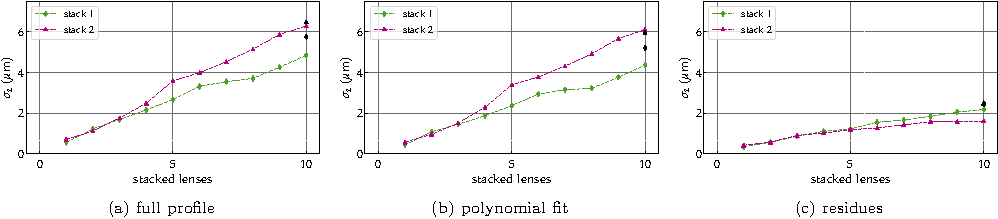
\includegraphics[width=1.\linewidth]{figures/ch04b/stacking_errors.pdf}}
%     \caption[Accumulative figure errors]{Progressive increase of figure errors for the (a) full-, (b) fit- and (c) residual- profiles. The green-diamond shaped marker indicates the artificially stacked lenses from the stack 1, while the magenta triangles, the stack 2. The black markers indicate the corresponding measured stack. Figure errors calculated for a geometric aperture of $A_{\diameter}=400~\mu\text{m}$.}
%     \label{fig:stacking_errors}
% \end{figure}

% \clearpage

\begin{table}[t]
\caption[Lens stack 1 main parameters from XSVT metrology]{Compilation of radii, figure errors and clear aperture for lenses L01 to L10 (stack 1) obtained with XSVT metrology.}
\centering
\label{tab:CDn}\small
% \resizebox{\columnwidth}{!}{
\begin{tabular}{cccccc}
\hline \hline
\textbf{lens}      & \textbf{radius}  & \multicolumn{3}{c}{figure errors$^\dagger$ (r.m.s) $\mu$m}  & \textbf{useful aperture}\\ \cline{3-5}
\textbf{number}    & $\mu$m           & full profile & pol. fit   & residues & $\mu$m\\ \hline
L01                &48.77   &0.57   &0.45   &0.35      &439\\
L02                &48.24   &0.80   &0.69   &0.43      &442\\
L03                &48.76   &0.77   &0.55   &0.54      &432\\
L04                &49.20   &1.05   &0.92   &0.51      &435\\
L05                &48.41   &0.81   &0.67   &0.44      &440\\
L06                &48.70   &1.07   &0.72   &0.79      &443\\
L07                &48.91   &0.70   &0.53   &0.46      &442\\
L08                &49.23   &0.84   &0.62   &0.56      &447\\
L09                &48.09   &0.93   &0.79   &0.49      &434\\
L10                &48.10   &0.88   &0.76   &0.44      &431\\
\hline
\multicolumn{2}{r}{\textbf{accumulated}:}      &4.84       &4.36  &2.18 &400\\
\hline
Stack 01:           &5.46   &5.75   &5.20   &2.47    &399\\
\hline \hline
\multicolumn{6}{r}{\footnotesize{$^\dagger$ values given for $A_{\diameter}=400~\mu\text{m}$}}     
% \multicolumn{2}{r}{\textbf{quadrature-sum}:}   &    &   &   &  & & $-$\\
\end{tabular}
% }
\end{table}

\begin{figure}[!htb]
    \centering
    {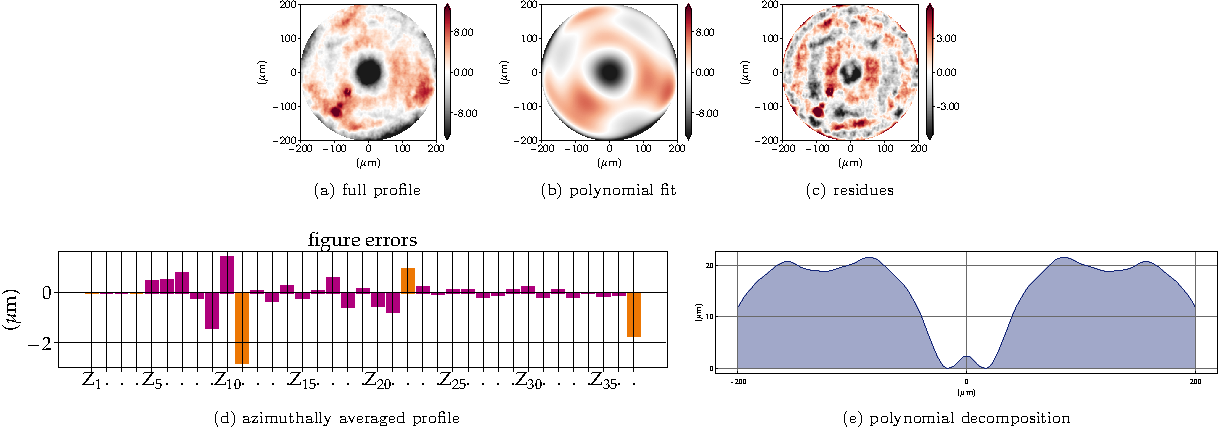
\includegraphics[width=1.\linewidth]{figures/ch04b/CDn_individual.pdf}}
    \caption[Figure errors from the artificially stacked lenses - L01-L10]{Individually measured and artificially stacked lenses forming the stack 1. The individual lenses parameters are shown in Table~\ref{tab:CDn}. Profiles calculated for a geometric aperture of $A_{\diameter}=400~\mu\text{m}$.}
    \label{fig:accumulated_profile_1}
\end{figure}

\begin{figure}[!htb]
    \centering
    {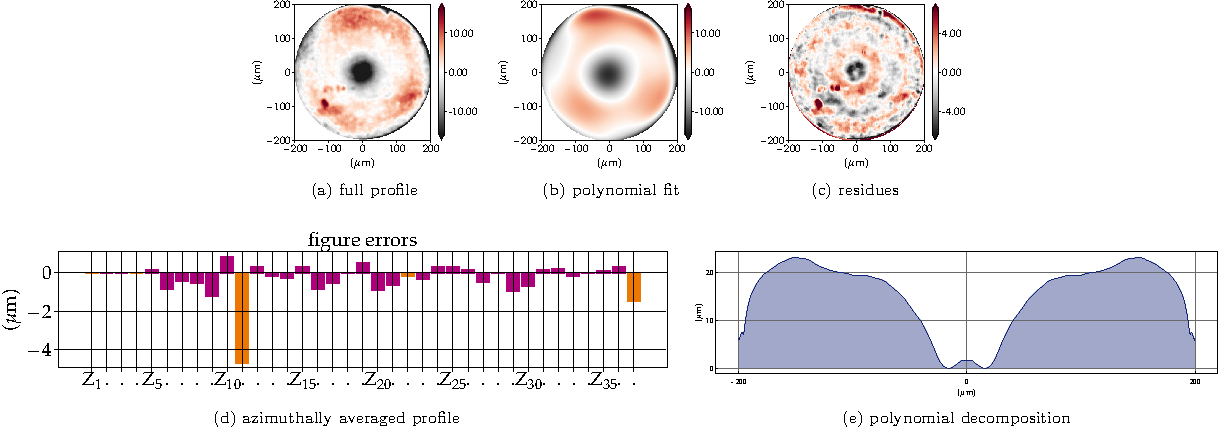
\includegraphics[width=1.\linewidth]{figures/ch04b/CDn_Stack.pdf}}
    \caption[Figure errors from stack 1]{Measurement of a CRL composed of the lenses L01-L10 described in Table~\ref{tab:CDn} (stack 1). Profiles calculated for a geometric aperture of $A_{\diameter}=400~\mu\text{m}$.}
    \label{fig:CDn}
\end{figure}

% \clearpage

\begin{table}[t]
\caption[Lens stack 2 main parameters from XSVT metrology]{Compilation of radii, figure errors and useful aperture for lenses L11 to L20 (stack 2) obtained with XSVT metrology.}
\centering
\label{tab:CDo}\small
% \resizebox{\columnwidth}{!}{
\begin{tabular}{cccccc} \hline \hline
\textbf{lens}      & \textbf{radius}  & \multicolumn{3}{c}{figure errors$^\dagger$ (r.m.s) $\mu$m}   & \textbf{useful aperture}\\ \cline{3-5}  
\textbf{number}    & $\mu$m           & full profile & pol. fit   & residues                                         & $\mu$m\\ \hline
L11                &49.05   &0.71   &0.57   &0.43      &440\\
L12                &49.27   &0.80   &0.68   &0.44      &460\\
L13                &48.98   &0.94   &0.75   &0.56      &435\\
L14                &48.26   &1.06   &0.95   &0.47      &452\\
L15                &48.25   &1.44   &1.36   &0.46      &444\\
L16                &49.25   &0.69   &0.55   &0.42      &443\\
L17                &48.94   &0.72   &0.61   &0.39      &433\\
L18                &48.30   &1.22   &1.15   &0.42      &439\\
L19                &47.78   &1.24   &1.21   &0.25      &419\\
L20                &48.62   &0.80   &0.72   &0.36      &456\\
\hline
\multicolumn{2}{r}{\textbf{accumulated}}      &6.28    & 6.10  &1.62 &400\\
\hline
Stack 02:           &5.67    &6.47   &5.97   &2.49  &407\\
\hline \hline
\multicolumn{6}{r}{\footnotesize{$^\dagger$ values given for $A_{\diameter}=395~\mu\text{m}$}}       
% \multicolumn{2}{r}{\textbf{quadrature-sum}:}   &    &   &   &  & & $-$\\
\end{tabular}
% }
\end{table}

\begin{figure}[ht]
    \centering
    {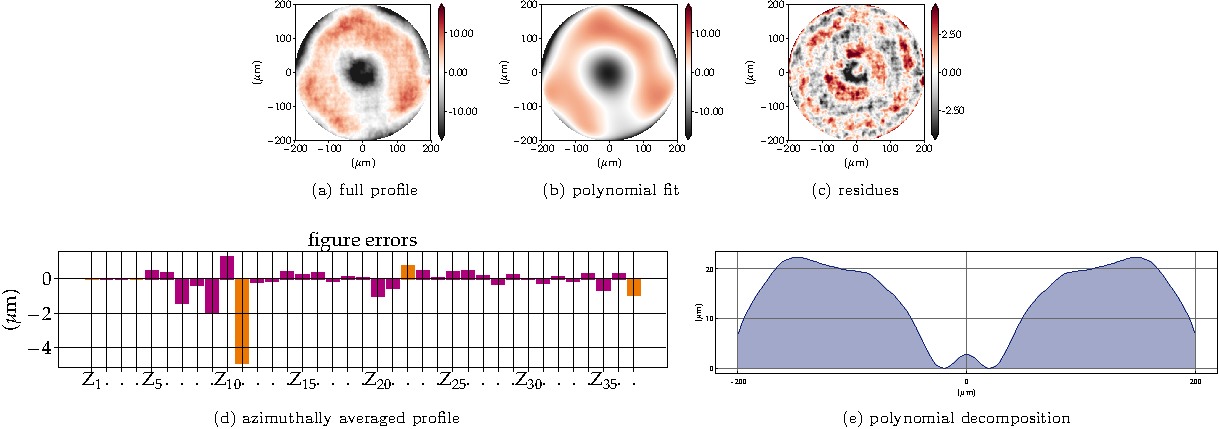
\includegraphics[width=1.\linewidth]{figures/ch04b/CDo_individual.pdf}}
    \caption[Figure errors from the artificially stacked lenses - L11-L20]{Individually measured and artificially stacked lenses forming the stack 2. The individual lenses parameters are shown in Table~\ref{tab:CDo}. Profiles calculated for a geometric aperture of $A_{\diameter}=400~\mu\text{m}$.}
    \label{fig:accumulated_profile_2}
\end{figure}

\begin{figure}[ht]
    \centering
    {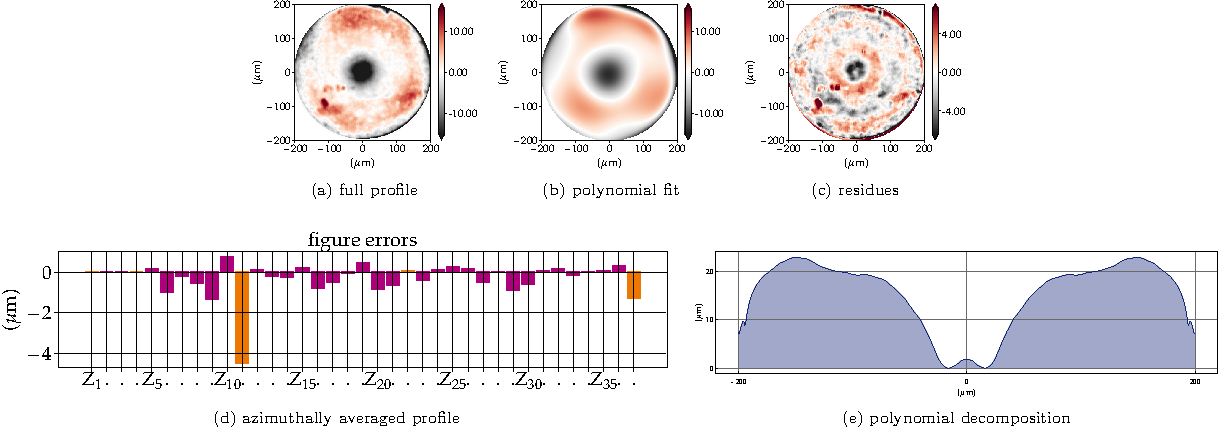
\includegraphics[width=1.\linewidth]{figures/ch04b/CDo_Stack.pdf}}
    \caption[Figure errors from stack 2]{Measurement of a CRL composed of the lenses L11-L20 described in Table~\ref{tab:CDn} (stack 2). Profiles calculated for a geometric aperture of $A_{\diameter}=400~\mu\text{m}$.}
    \label{fig:CDo}
\end{figure}


% \clearpage

\begin{figure}[ht]
        \centering
        {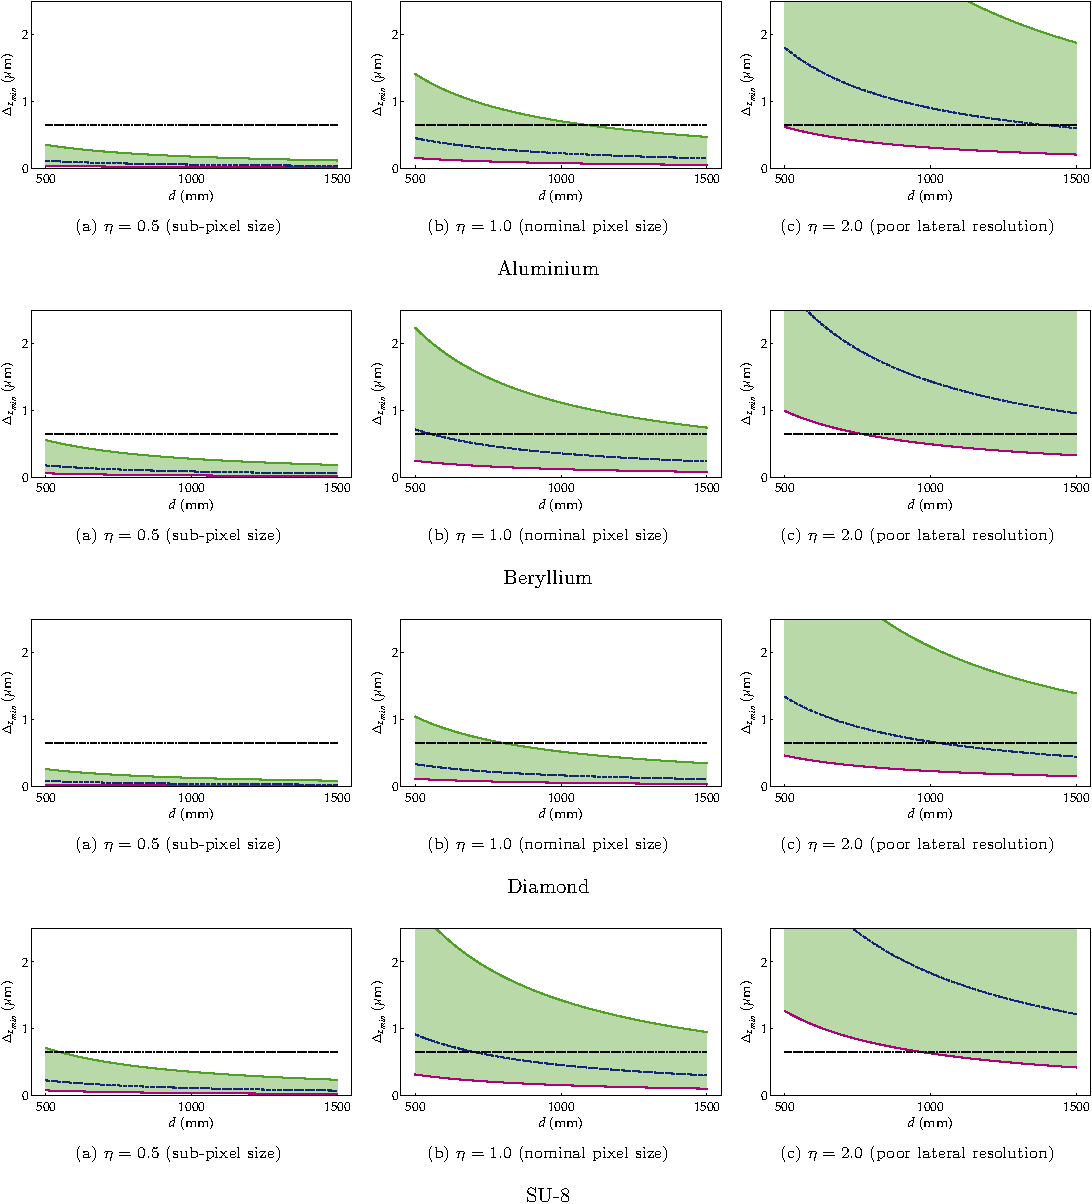
\includegraphics[width=1.0\linewidth]{figures/ch04b/sensitivity_2.pdf}}
        \caption[XSVT sensitivity calculation]{X-ray speckle vectorial tracking longitudinal sensitivity ($\Delta{z_{\text{min}}}$) for four common used materials for refractive optics manufacturing. The solid red line indicates the performance of the method at 10~keV, while the solid green line for 30~keV. The dashed purple line indicates the experimental performance at 17~keV (used energy for such experiments in this work.). Black point-dashed line indicates the nominal pixel size of the imaging detector $\Delta_\text{pixel}=0.65~\mu$m. Curves calculated using Eq.~\ref{eq:XSVT_resolution}.}\label{fig:sensitivity_2}
\end{figure}

\clearpage

\addcontentsline{toc}{section}{References}
\printbibliography[heading=subbibliography]
\end{refsection}

% % Backup from discussion with Seb:

% berujon: Here the question is more mathematical than physics or geometrical. You have a gradient function and you can assume for each point an error \sigma on this measurment. You can next assume all the point error have the same distribution and are decorrelated. Then the error on the surface by integration between two projected points/pixel is \sigma * int_step (ici en general la taille de pixel). \delta comes somewhere here to scale from wavefront to lens surface. Now, if you integrate a full line (i.e. with cumsum), playing with the math around the "propagation of uncertainty", you'll get un error on the function \sqrt(N)* \sigma * int_step. So for big lens it can multiply up to 45. This is what you see within the first papers on grating interferometry in 1D. Check Irene Zanette paper also on the first 2D interferometer. But good thing is that we are using
% berujon: 2D integration with speckle since we have 2D gradients and the error cancel out each other. For a Zonal reconstruction/integration check Southwell @article{RN235, author = {Southwell, W. H.}, title = {Wave-front estimation from wave-front slope measurements}, journal = {J. Opt. Soc. Am.}, volume = {70}, number = {8}, pages = {998-1006}, url = {http://www.opticsinfobase.org/abstract.cfm?URI=josa-70-8-998}, year = {1980}, type = {Journal Article} }
% berujon: The guy did the math. Harker uses the same kind of integration but with regulariszation, so the factor should be more or less equivalent.
% berujon: @article{RN214, author = {Fried, David L.}, title = {Least-square fitting a wave-front distortion estimate to an array of phase-difference measurements}, journal = {J. Opt. Soc. Am.}, volume = {67}, number = {3}, pages = {370-375}, url = {http://www.opticsinfobase.org/abstract.cfm?URI=josa-67-3-370}, year = {1977}, type = {Journal Article} } also provided a formulae, you'll see it scales with the log of the number of pixel
% berujon: For Fourier integration, like the Frankot Chellapa algorithm, I don't really know.

% berujon: In such case do not hesitate: sin(\alpha) = \alpha, cos(\alpha) = 1
% berujon: Should be simply \delta pix *\alpha_min/delta. \eta should be only for the precision of the tracking of \nu

% berujon: This would make good sense to do, to know the factor \eta. That will give you the error on the angle/defletion/gradient and then by integration you can infer the error on the surface.
% berujon: Check also quickly wikipedia on propagation of uncertainty and the composition of function
% berujon: You can either use the beginning and end of ref sets or a region with no sample if there is one


